\section{Background and related work}




In Mixture of Experts, although each expert receives all input variables, only a subset is truly relevant to the specific task assigned to the expert. This variable selection is frequently implicit, as each expert focuses on the most useful characteristics for its task. However, this selection can be made explicit through regularization mechanisms, such as $L_1$ \citep{courbariaux2022sparse}, $L_2$ \citep{jordan1994hierarchical}, or elastic net \citep{chamroukhi2019regularized, ma2018modeling}. For $K$ experts, this would be equivalent %to trying 
to maximize the following quantity:
%
\begin{align}
    \mathcal{L}(\bbeta,\bpi ; \by,\bX) &= \prod_{i=1}^N \sum_{k=1}^K \underbrace{g\left(\bX_i ; \bpi \right)_k}_{\text{Gating Network}}
   \underbrace{ f_k\left(y_i; \bX_i, \bbeta_k\right)}_{\text{Expert}} \notag
   \\ &\quad + \underbrace{\lambda \left( \alpha \sum_{k=1}^K \sum_{j=1}^p \lvert \pi_{kj} \rvert  + \dfrac{1-\alpha}{2}\sum_{k=1}^K \sum_{j=1}^p \pi_{kj}^2\right) }_{\text{Regularization terms}},
    %\sum_{\bZ \in \mathcal{Z}} \prod_{i=1}^N  \p\left(Z_i \mid \bX_i \right) \p\left( y_i \mid Z_i, \bX_i \right) & (probabilist modeling)
\end{align}
%
where $g\left(\bX_i ; \bpi \right)_k$ is the $k$-th output of the gating network detailed in Equation~\eqref{eq:g_k}, $\bpi$ are gating network parameters, $(\bbeta_k)_{k=1:K}$ are experts parameters, $\lambda>0$ is an hyperparameter linked to regularization strength and $\alpha>0$ is an hyperparameter for elastic-net regularization.

These regularizations, primarily applied to the gating network, enhance interpretability by controlling expert selection directly. The gating network plays a central role in variable and expert selection, and different approaches can be classified into three main categories \cite{cai2024survey}: dense \citep{wu2023mole, pan2024dense}, sparse \citep{jiang2024mixtral, tan2023sparse, zhou2022mixture}, and soft \citep{puigcerver2023sparse, zadouri2023pushing}. 

In sparse methods, regularizations are designed to activate a limited number of experts or variables, which improves the interpretability by aligning predictions with the variables involved \citep{zhou2022mixture}. 
The main approach is to use the top-$L$ experts, meaning the $L$ experts with the highest values according to the gating network:
%
in general, the gating network $g$ is composed of $(g_k)_{k=1:K}$ functions, and is defined as
\begin{equation}
    g(\bX_i ; \bpi) = \softmax \left(g_1\left(\bX_i ; \bpi_1 \right), \cdots, g_K\left(\bX_i ; \bpi_K \right) \right). 
\end{equation}
Typically, to limit the number of activated experts, according to \cite{cai2024survey}, the gating network output $g(\bX_i)_k$ is replaced by:
\begin{equation}
\label{eq:g_k}
    \tilde{g}(\bX_i)_k = \softmax\left(\operatorname{TopL}\left( g_1\left(\bX_i; \bpi_1\right) \right),\cdots,\operatorname{TopL}\left(g_K\left(\bX_i; \bpi_K\right)\right) \right)_k,
\end{equation}
where 
\begin{equation}
    \operatorname{TopL}(g_k(\bX_i; \bpi)) = \left\{
    \begin{array}{ll}
        g_k(\bX_i; \bpi) & \mbox{if } g(\bX_i; \bpi)_k \in \text{top-L elements of } g(\bX_i; \bpi), \\
        -\infty & \mbox{else.} 
    \end{array}
    \right.
\end{equation}
%
Currently, sparse MoEs typically refers to limiting the number of active experts, thereby reducing computational cost. However, an increased specialization among a large pool of experts does not necessarily ensure sparsity in terms of variable selection.
%
On the other hand, soft approaches allow more gradual and partial expert activation, offering a balance between sparsity and flexibility. 
All MoEs with regularization mechanisms on the gating network fall into this class of models. 
While these models achieve sparsity in terms of variable selection, they remain soft in terms of expert activation. Indeed, it is not always possible to ensure that only a minimal subset of experts will be activated.
%This may limit their ability to produce entirely sparse solutions in terms of the experts selected.

The integration of these penalties structures the gating network's behavior and encourages a parsimonious selection of variables. This simplifies interpretation by reducing the number of variables and experts involved in decision-making, while maintaining computational efficiency \citep{shazeer2017outrageously}. However, the separation between variables used by the gating network and those leveraged by experts in the final prediction can complicate the interpretability, as the most influential variables for selection are not always the most relevant for prediction. This disjunction introduces a potential bias in model interpretation.
Several efforts have been made to improve the interpretability of MoEs, for instance:
\begin{itemize}
    \item \cite{ismail2022interpretable} developed an interpretable MoE model, introducing an approach that makes expert decisions more transparent by employing explanation techniques such as assignment modules and studying expert contributions.
    \item Since 2017, the integration of attention mechanisms in MoEs, as presented by \cite{shazeer2017outrageously}, has made the decision process more explicit by focusing the model's attention on specific aspects of the data. Additionally, this work introduced the concept of the MoE-layer, which has been widely reused in recent Deep Learning architectures \citep{lepikhin2020gshard, fedus2022switch, zhou2022mixture}.
    \item In the context of Multitask Learning, \cite{ma2018modeling} proposed using multiple gating networks, linked to the associated prediction tasks, providing a clearer connection between the experts utilized, the gating network predictions, and the final outcomes.
\end{itemize}

Ensuring interpretability is an important aspect in machine learning applied to sensitive areas. In Mixture Of Experts framework, which can be achieved not only through the design of the gating mechanism but also by employing interpretable experts. Experts based on linear regression are a common choice in this regard, as they allow for a clear justification of the decisions made by each expert. Moreover, experts based on linear regression are often favored due to their computational efficiency.

These type of Mixture of Experts models generally fall within the category of Latent Regression Models (LRMs), where the experts are based on latent subpopulations, and the regression coefficients capture subgroup-specific effects \citep{vermunt2002latent, desarbo1988maximum}.
More specifically, the general model is often defined as follows:
\begin{align}
    \bZ_i &\sim \M\left(1; \bpi = \left(\pi_1, \cdots, \pi_K\right) \right), \\
    y_i \mid \bX_i, Z_{ik}=1 &\sim \mathcal{N}\left(\bX_i \bbeta_k, \sigma^2_k\right),
\end{align}
where $\bZ_i$ is a latent variable for expert allocation for observation $i$ and $\bbeta_k$ are regression parameters for the $k$-th expert (or community).

In this framework, the role of the gating network is associated with the variable $Z$. This variable refers to community membership, it is assumed that individuals from the same cluster are studied by the same expert.


Nevertheless, several extensions have been developed, including longitudinal data models and co-clustering regression models.

\paragraph{Longitudinal data models:} Individuals within the same community share similar dynamics over time. Each latent class has its own risk profile for the event under study or its own longitudinal pattern \citep{proust2014joint, courbariaux2022sparse}.
Following the model of \cite{courbariaux2022sparse}, and with our notations, we would have :
\begin{align}
    \bZ_i &\sim \M\left(1; \softmax\left(\bX_i \bpi \right)\right), \\
    y_{iv} \mid \bX_i, \mathbf{T}_i, Z_{ik}=1 &\sim \mathcal{N}\left( \sum_{r=1}^R  \beta_{kvr} T_{iv}^r , \sigma^2_{vk}\right).
\end{align}
In this context, $\bX$ is considered as a $N \times p$ matrix. The latent variable is obtained by a multiclass regression parameterized  by a $p \times K$ matrix $\bpi$.
On the $v$-th visit and for the community $k$, the polynomial regression is parameterized by $\bbeta_{kv}$, and $T_{iv}$ is the time metric (the
patient’s age or time since the disease was first diagnosed, for instance).
 
\paragraph{Co-clustering Regression Model:} \cite{vu2015variational} proposed a multitask regression algorithm based on an \textit{LBM} partitioning of the $N \times p$ label matrix $\mathbf{y}$.
Each block of the matrix is associated with regression parameters for the covariates $\bX$. The Latent Block Regression Model (\textit{LBRM}) developed by \cite{boutalbi2022latent} extends this by partitioning the $N \times p \times d$-tensor $\bX$ based on the same stratification as the label matrix $\mathbf{y}$. The last dimension of the tensor $\bX$ corresponds to the covariates used in the regression.
More precisely, and with our notations :
%
\begin{align}
    \bZ_i &\sim \M\left(1; \bpi = \left(\pi_1, \cdots, \pi_K\right) \right), \\
    \bW_j &\sim \M\left(1; \brho = \left(\rho_1, \cdots, \rho_Q\right) \right), \\
    y_{ij} \mid \bX_{ij}, Z_{ik}=1, W_{js}=1 &\sim \mathcal{N}\left(\bX_{ij} \bbeta_{ks}, \sigma^2_{ks}\right).
\end{align}
 For an observation \( i \) belonging to community \( k \) and a problem \( j \) in category \( s \), a regression is performed along the third dimension, on $(\bX_{ijr})_{r=1:d}$, parameterized by a coefficient vector \( \bbeta_{ks} \in \mathbb{R}^d \).

In the supervised framework, we aim to achieve both interpretability and predictive performance. The objective of our approach is to incorporate an additional structure into the data used for prediction. While the stratification of individuals is already induced by the Mixture of Experts framework, we aim to extend this by also integrating a structure on the variables. Through a mixture model applied to covariates, the goal is to capture the emergence of both redundant information within components and complementary information between components. This approach mirrors the work on \textit{mimi-SBM}, which handles similar challenges but for multi-view clustering.

As illustrated in Figure \ref{fig: CoCoLBM_MNIST}, to obtain more specific partitions compared to a standard mixture model on covariates, a conditional stratification of variables, depending on the community structure, is needed. The resulting model, named Mixture Of Experts and BIclustering Unified Strategy (\textit{MoEBIUS}), merges MoEs with a conditinal biclustering algorithm to offer precise predictions alongside clear interpretation of latent communities and components.

More specifically, the model summarizes the components into a representative variable for each, then performs a regression on these representations, where the regression parameters depend on the community to which the observation belongs, an illustration of MoEBIUS is provided in Figure \ref{fig: CocoLBMoE}.

\begin{figure}[!ht]
     \centering
     \begin{subfigure}[b]{0.49\textwidth}
         \centering
         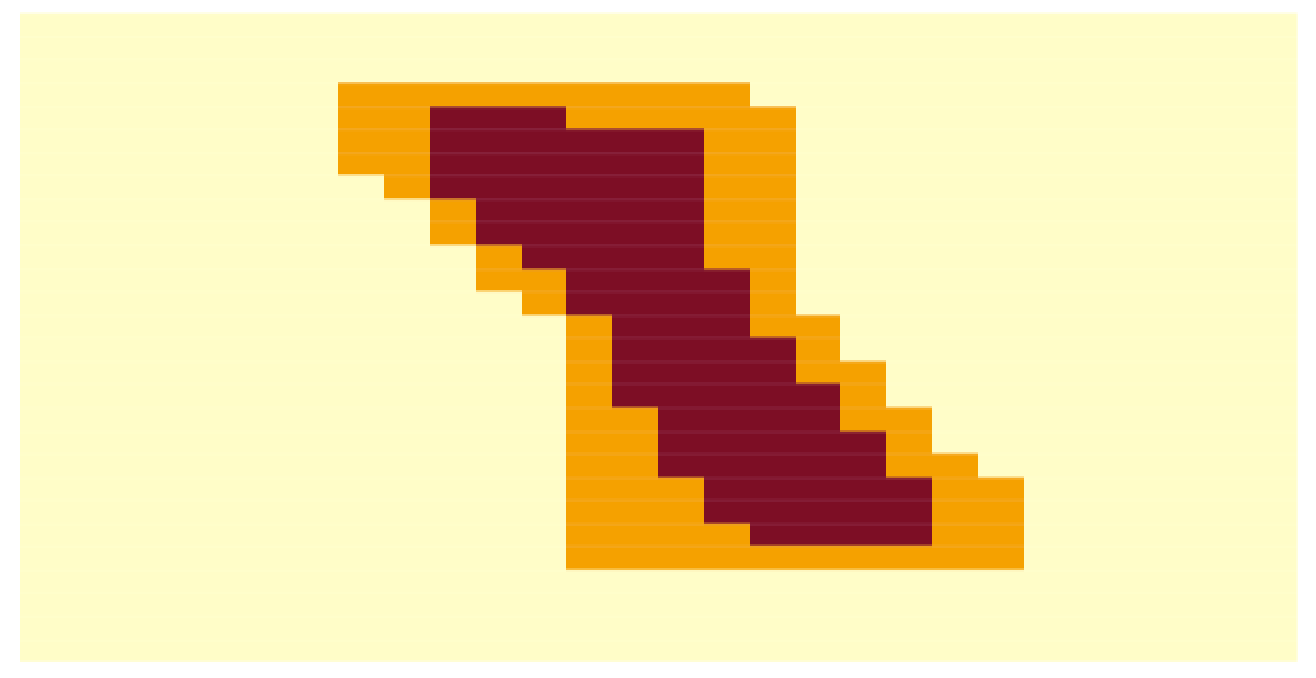
\includegraphics[width=\textwidth]{Figures/MNIST_LBM.png}
         \vspace{1.6cm}
         \caption{}
     \end{subfigure}
     \hfill
     \begin{subfigure}[b]{0.49\textwidth}
         \centering
         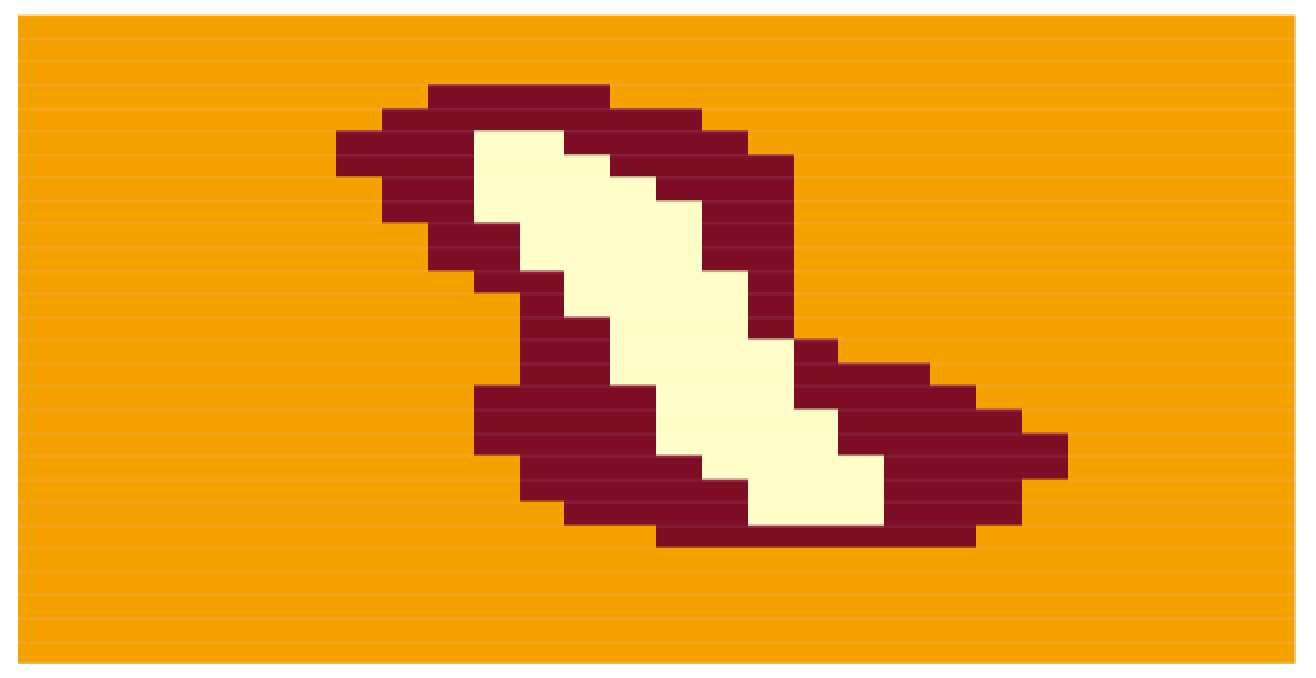
\includegraphics[width=\textwidth]{Figures/MNIST_cocoLBM_1.png}
         \caption{}
         \centering
         
\includegraphics[width=\textwidth]{Figures/MNIST_cocoLBM_8.png}
         \caption{}
     \end{subfigure}
     \caption{Different component partitions on MNIST data for digits $1$ and $8$. Figure (a) shows a partition defined by an \textit{LBM}, where the overall shape of both digits is captured. Figures (b) and (c) are derived from the \textit{Conditional LBM} \citep{goffinet2020conditional}, where the partitioning of variables depends on the observations (i.e., the digits). For each partition, the key pixels of interest specific to each digit are more clearly identified.}
     \label{fig: CoCoLBM_MNIST}
\end{figure}

% \kds{
% Our approach is inspired by the work on \textit{LBRM}, aiming to partition data using a latent block model to summarize information and then applying a regression model tailored to the stratification. To obtain a finer partition than that from an LBM, we adopt the Conditional Latent Block Model approach developped by \cite[][CLBM]{goffinet2020conditional} . The combination of Mixture of Experts and biclustering algorithms has led to the development of the model presented below, named Mixture Of Experts and BIclustering Unified Strategy (\textit{MoEBIUS}).}{Dire plutôt qu'en voulant faire interpretation + perfs., partir cadre modèle d'experts, apport aspect cond. à la stratification. Remettre dans le contexte du MoEs.}


